\documentclass[../ProjectDocumentation.tex]{subfiles}
%Gummi|065|=)
\title{\textbf{Processor Documentation}}
\author{Yuntong Lu, formatted by Kyle Lemmon}
\date{}
\graphicspath{{../}}
\begin{document}

\maketitle

\subsection{Datapath}
Inside of the data path, we connect ALU, regfile, Program counter and memory as the picture
shows.
For the ALU, the input values come from regfile. The result will go to a MUX. The flags values
will be sent to Flag block. Flag block stores 5bit flags. From the lower bit to higher bit, the flags
are CLFZN.
For the Regfile, the input comes form a MUX and FSM. MUX will choose either ALU result or
Memory out. The FSM controls the reset of the input’s ports. The outputs will go to ALU,
Program counter and Memory.
For the Program counter, the ld\_pc value is rd2 value which comes from Regfile. The other
inputs come from FSM. The output will go to a MUX.
For the Memory, the inputs come from either rd2 or pc value. The pc value decides the address
value. rd2 value decide the data port. The rest of the input ports come from FSM. The output
value will send to a MUX. Fig. \ref{fig:datapath} shows the datapath.
\begin{figure}
\centering
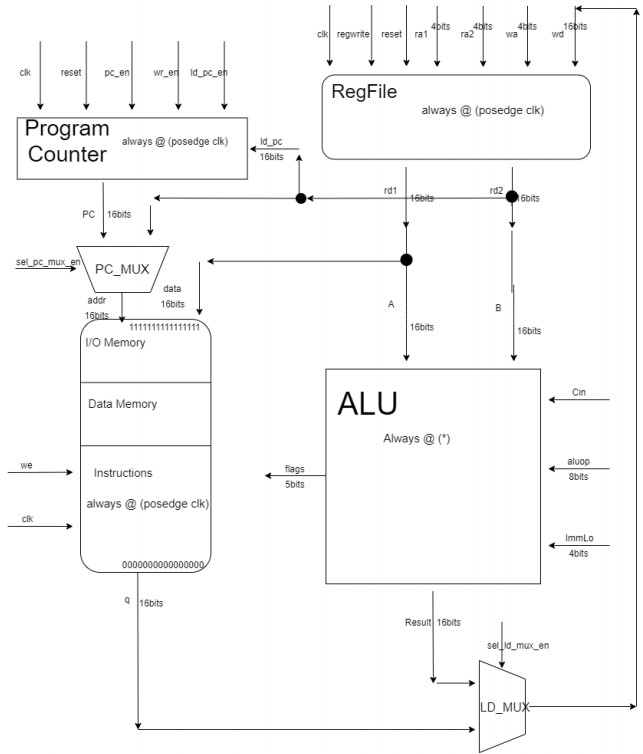
\includegraphics[width=12cm]{datapath}
\caption{Input and output of the program counter module.}
\label{fig:datapath}
\end{figure}
\subsection{ALU}
ALU will take care of all the calculate part. The 8 bit aluop will be the {OPCODE[15:12],
OPCODE[7:4]}. Depend on the aluop, the ALU would know which calculation needs to perform.
The immediate value has two parts. The IMMHI part will be included into aluop, and IMMLO
part will be directly sent to ALU. ALU will also compare the values while calculating them. The
flags will be raised depend on the values. Fig. \ref{fig:alu} shows the ALU.
\begin{figure}
\centering
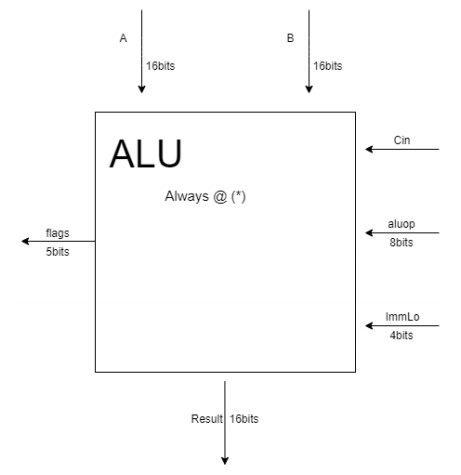
\includegraphics[width=8cm]{alu}
\caption{Input and output of the program counter module.}
\label{fig:alu}
\end{figure}
\subsection{Register File}
Regfile has 16 reg spaces. Each reg space can store 16 bit values. At the posedge of the clock,
the value will be written or read. ra1 and ra2 controls the selected address. The regfile has two
port outputs, the rd1 and rd2. They can be read together. When the regwrite is enabled, the value
will be written to the regfile, the output will be the written value. Fig. \ref{fig:regfile} shows the register file.
\begin{figure}
\centering
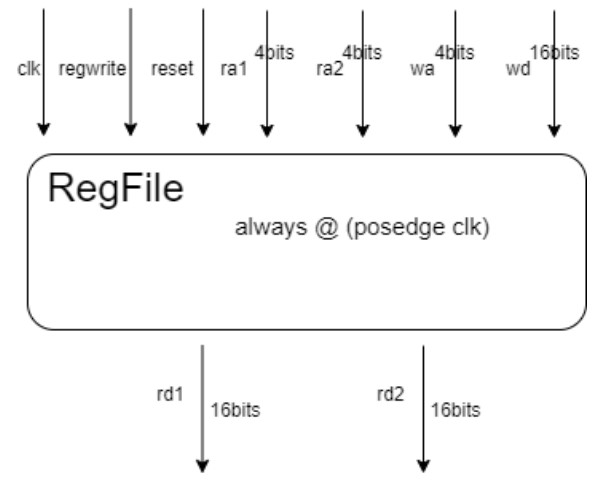
\includegraphics[width=8cm]{regfile}
\caption{Input and output of the program counter module.}
\label{fig:regfile}
\end{figure}
\subsection{Program Counter}
Program counter has one output pc. The output has three different sources. The first is when
pc\_en is on, ld\_en and wr\_pc is off, the pc value will pulse 1 at each posedge of the clock. When
pc\_en and ld\_en is on, the pc value will be current pc value pulse ld\_pc at each posedge of the
clock. When pc\_en and wr\_en is on, the pc value will be overwritten to ld\_pc value at the
posedge of the clock. We can use it to perform JCOND and SCOND by changing the value of
ld\_pc. Fig. \ref{fig:pc} shows the program counter.
\begin{figure}
\centering
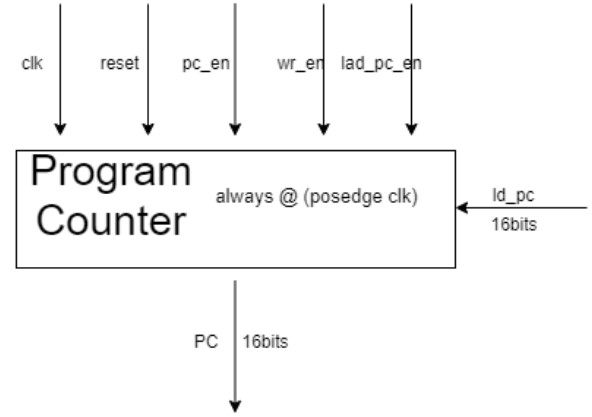
\includegraphics[width=8cm]{pc}
\caption{Input and output of the program counter module.}
\label{fig:pc}
\end{figure}

\subsection{Memory}
Memory is generated from templet. add will decides the address. we means write enable, data
port will be used when write the new data into the memory. The memory will store instructions
from the address 0. The total space is 65535. Each space stores 16bit values. The assembler will
decide how to use the memory. Fig. \ref{fig:memory} shows the memory module.
\begin{figure}
\centering
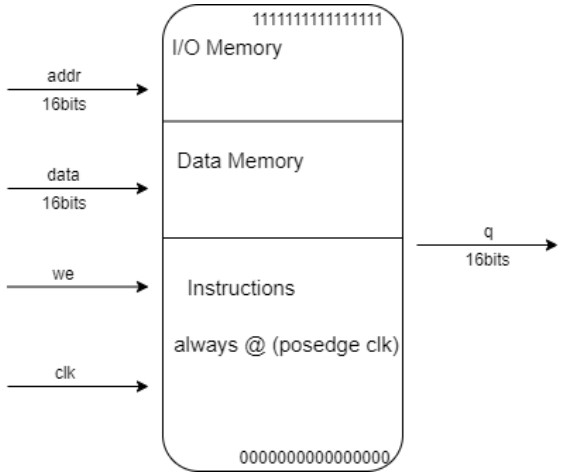
\includegraphics[width=8cm]{memory}
\caption{Input and output of the program counter module.}
\label{fig:memory}
\end{figure}

\subsection{Control FSM}
FSM controls almost all the data path input ports. It just needs the flag information and
instructions in the jump conditions. FSM decide when to open and how long to open the port.
In the FSM, I put lots of states in here. The states are depending on the instructions. Same with
ALU, each instruction has its own state. But the state can be separate into three major part. First
is regToreg, which means the value comes from register and goes to register. Second is
regTomem, which means the value comes from register or memory and goes to the other side.
The third is immediate values, the value comes from instructions and the result goes to register.
At the posedge of the clock, the state will update to the next state. At the negedge of the clock,
the output value will be decided in the state.
For the regToreg and immediate states, it takes 1 clock cycle to finish the job. For the store
instruction, it takes 3 clock cycles. For the load instructions, it takes 4 clock cycles, for the jump
instructions, it take 3 clock cycles. Fig. \ref{fig:fsm_diag} shows the processor control module, and Fig. \ref{fig:fsm} shows the state diagram for the control module.

\begin{figure}
\centering
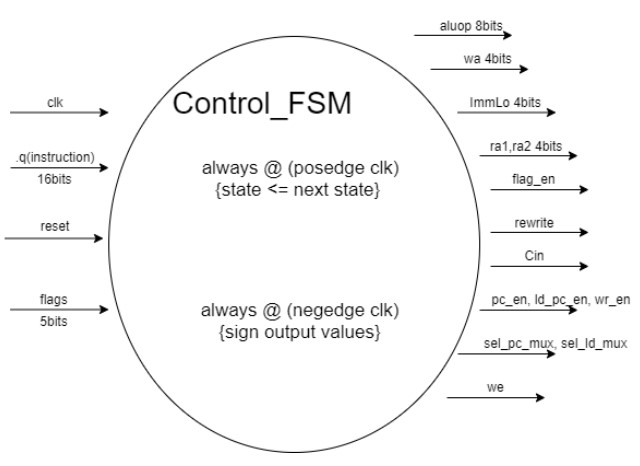
\includegraphics[width=10cm]{fsm_diag}
\caption{Input and output of the program counter module.}
\label{fig:fsm_diag}
\end{figure}

\begin{figure}
\centering
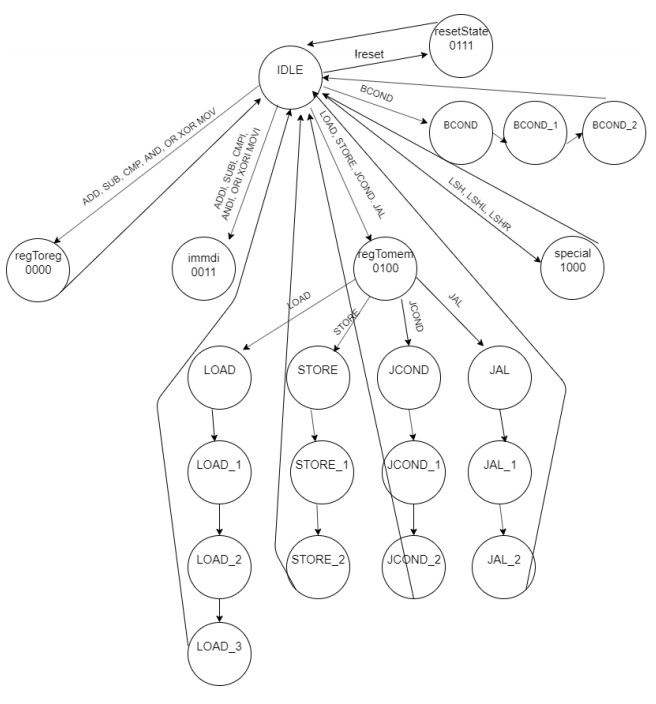
\includegraphics[width=12cm]{fsm}
\caption{Input and output of the program counter module.}
\label{fig:fsm}
\end{figure}

\end{document}
